%%%%%%%%%%%%%%%%%%%%%%%%%%%%%%%%%%%%%%%%%
% fphw Assignment
% LaTeX Template
% Version 1.0 (27/04/2019)
%
% This template originates from:
% https://www.LaTeXTemplates.com
%
% Authors:
% Class by Felipe Portales-Oliva (f.portales.oliva@gmail.com) with template 
% content and modifications by Vel (vel@LaTeXTemplates.com)
%
% Template (this file) License:
% CC BY-NC-SA 3.0 (http://creativecommons.org/licenses/by-nc-sa/3.0/)
%
%%%%%%%%%%%%%%%%%%%%%%%%%%%%%%%%%%%%%%%%%

%----------------------------------------------------------------------------------------
%	PACKAGES AND OTHER DOCUMENT CONFIGURATIONS
%----------------------------------------------------------------------------------------

\documentclass[
	12pt, % Default font size, values between 10pt-12pt are allowed
	%letterpaper, % Uncomment for US letter paper size
	%spanish, % Uncomment for Spanish
]{fphw}

% Template-specific packages
\usepackage[utf8]{inputenc} % Required for inputting international characters
\usepackage[T1]{fontenc} % Output font encoding for international characters
\usepackage{mathpazo} % Use the Palatino font
\usepackage{subcaption}
\usepackage{siunitx}
\usepackage{graphicx} % Required for including images
\graphicspath{{figures}]}
\usepackage{booktabs} % Required for better horizontal rules in tables
\usepackage{epstopdf} %converting to PDF
\usepackage{listings} % Required for insertion of code
\usepackage{hyperref}
\usepackage{enumerate} % To modify the enumerate environment
\usepackage{todonotes}
\usepackage[numbers]{natbib}
%----------------------------------------------------------------------------------------
%	ASSIGNMENT INFORMATION
%----------------------------------------------------------------------------------------

\title{Study of water self-diffusion between walls} % Assignment title

\author{Matteo Finco} % Student name

\date{September, 2022} % Due date

\institute{Università degli studi di Padova, Dipartimento di Scienze Chimiche} % Institute or school name

\class{COMPUTATIONAL METHODS FOR MATERIALS SCIENCE} % Course or class name

\professor{Alberta Ferrarini} % Professor or teacher in charge of the assignment

%----------------------------------------------------------------------------------------

\begin{document}
\bibliographystyle{plainnat} 
\maketitle % Output the assignment title, created automatically using the information in the custom commands above

%----------------------------------------------------------------------------------------
%	ASSIGNMENT CONTENT
%----------------------------------------------------------------------------------------

\section*{Abstract}
A particularly suitable application of Molecular Dynamics, is the study of nanofluid systems. In this report, the effects on structure and dynamics of water between two walls is discussed to correlate the varying distance between the walls and the reduced self-diffusion observed.
Lastly, considerations about the anisotropy introduced by the presence of walls are formulated on the basis of the extrapolated bulk diffusion coefficient for the different axis.

%----------------------------------------------------------------------------------------

\section{Introduction}
Molecular Dynamics (MD) consists in a computational technique which exploits the use of classical potentials to simulate the interactions between components of the desired system.
This caveat allows to greatly expand the accessible length of the trajectories and size of the system when compared to quantum mechanical methods such as Density Functional Theory (DFT).
This is made possible by a classical approach that relies on statistical thermodynamics to guide the system through physically meaningful trajectories in the phase space (eq.\ref{phase-space}) and describes the kinetics of individual components following Newtonian mechanics, eq.\ref{Newton}, which establishes the observable properties of the simulation.
\begin{equation}
	E = H (\textbf{p}^{N}, \textbf{r}^{N})
	\label{phase-space}
\end{equation}
\begin{equation}
	\textbf{F}_{i} = -\frac{\delta V(\textbf{r}_{1}, \textbf{r}_{2},..., \textbf{r}_{i},..., \textbf{r}_{n})}{\delta \textbf{r}_{i}}
	\label{Newton}
\end{equation}
Thermodynamic and mechanic considerations are linked by a postulate, which states that thermodynamic properties can be extrapolated as time averages of the observables in a microscopic system, as expressed in eq.\ref{postulate} .
\begin{equation}
	\langle f\rangle = \lim\limits_{T \to \infty} \frac{1}{T} \int_{0}^{T} f(\textbf{r}^{N}(t),\textbf{p}^{N}(t)) dt 
	\label{postulate}
\end{equation}
Constraints on the evolution of the system are set by the applied ensemble, which is a set of thermodynamic properties that is kept constant during the simulations.
When simulating dynamic properties, either the $NVE$ micro-canonical ensemble\cite{mark_structure_2001} or the isothermal-isobaric ensemble\cite{jorgensen_comparison_1983} can be employed.
However, the simplification of the interactions necessary to treat classically a system on the molecular scale comes at the cost of accuracy since the specific interactions are appointed arbitrarily through classical fields.
For this reason, systems often recurring in literature, such as water, have been modeled in a great number of ways to better fit the specific purpose of some studies or to increase consistency with experimental findings.\cite{tsimpanogiannis_self-diffusion_2019}
For example, TIP3P\cite{jorgensen_comparison_1983} model represents a reparametrization of the O-O interactions to better fit to the experimental data of the radial distribution function.
Later, the very same model has been updated to feature the Ewald summation rather than short nonbonded truncation schemes.\cite{price_modified_2004}
Moreover, the use of Molecular Dynamics has acquired great relevance in the simulation of confined fluids.
In the work of \citet{yeh_system-size_2004}, they arrive to the expression of the relation between the diffusion coefficient for bulk fluids and quantity estimated by applying Periodic Boundary Conditions (PBD), as reported in Eq.\ref{Dpbc}.
\begin{equation}
	D_{PBC} = D_{0} - \frac{k_{B}T\xi}{2d \pi \eta L}
	\label{Dpbc}
\end{equation}
In this equation, $D_{PBC}$ is the diffusion coefficient calculated from calculations running on a unit cell replicated by PBCs, $D_{0}$ is the bulk diffusion coefficient of the fluid, $k_{B}T$ is the thermal quantum, $\xi$ is a constant related to the Ewald summation, $d$ is the number of dimensions in which the unit cell is limited, $\eta$ is the viscosity and $L$ is the size of the unit cell.
Such relationship allows the extrapolation of the bulk diffusion coefficient from the intercept of the linear regression of the D(1/L) data with the $y$ axis.
Additionally, from the slope of such regression is possible to estimate the value of viscosity of the fluid.

%----------------------------------------------------------------------------------------
\section{Calculations and Results}
Calculations were run using the force fields and models provided by prof. Ferrarini using LAMMPS (version 4 May 2022).\cite{thompson_lammps_2022}
For the analysis of data the \texttt{lammps-thermo}\cite{ryan_s_defever_lammps_thermo_2021} package was used along with Python scripts\cite{matteo_finco_md_water_self_diffusion_2022}, analysis of the self-diffusion coefficient was performed on OriginPro 2018.
\subsection{Input files}
Periodic boundary conditions were allowed on all dimensions, while on the confined dimension trespassing was prevented by using a Lennard-Jones 9-3 potential set by the command:
\begin{verbatim}	
	fix	       zwall1 all wall/lj93 zlo EDGE 1.0 1.0 2.5 pbc yes
	fix	       zwall2 all wall/lj93 zhi EDGE 1.0 1.0 2.5 pbc yes
\end{verbatim}
This command places a wall that needs a sufficient amount of energy $\epsilon =$ 1 Kcal/mol to not be trespassed, a low enough  Van der Waals radius $\sigma = 1 \r{A}$ and cutoff distance $r_{cut} =$ 2.5 \r{A} to perturb excessively the system enclosed.
The box was set to allocate replicas of the water molecule with a 10x10 base, to offer enough statistical significance, while the height between 1 to 10 molecules.
Since the system was found to converge to realistic values of density, the interaction and execution parameters were not varied.
From an interaction point of view, this meant that the accuracy of long range interactions was kept to the $10^{-5}$ level and the force field was the updated version of TIP3P provided by \citet{price_modified_2004}.
Energy and force minimization for the first relaxation step was set to be achieved once they were stable, less than 1000 minimizing iterations and 10000 force-energy evaluations were sufficient  in all cases.
Velocity distributions were created at 300 K using as seed 1298371.
The execution of the simulations required the application of the isothermal-isobaric ensemble in stable conditions, first for $10^{3}$ equilibration steps and the for $10^{5}$ production steps, in order to keep the simulated water at 300 K and 1 atm.

\subsection{Results}
The trajectories were first analyzed to verify the thermodynamic stability of the simulation. 
All simulations were stable in temperature and total energy with deviations within 4 \% margin, see Fig. \ref{log}.\\

\begin{figure}[h!]
	\centering
	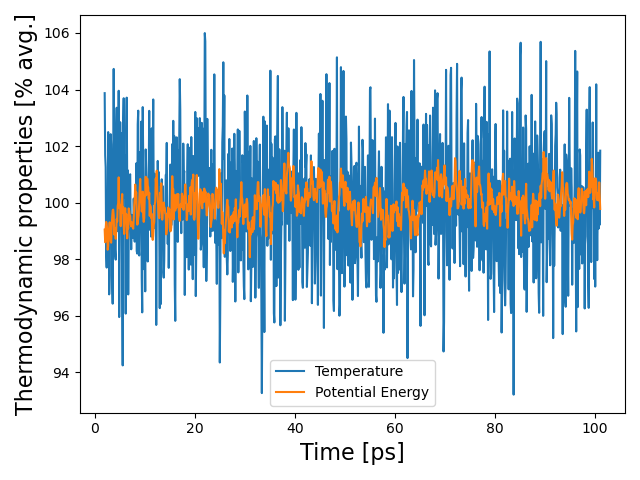
\includegraphics[width=0.6\textwidth]{log 8}
	\caption{Plot of temperature and potential energy deviations during the simulation of water between two walls 25 \r{A} apart from each other.}
	\label{log}
\end{figure}
\subsubsection{Structure and confinement}
Furthermore, the effect of confinement on radial distribution function and the density profile across the section of the two walls were calculated and a sample of the acquired data can be seen in Fig. \ref{g-rho}.
\begin{figure}[h!]
	\centering
	\begin{subfigure}{0.4\textwidth}
		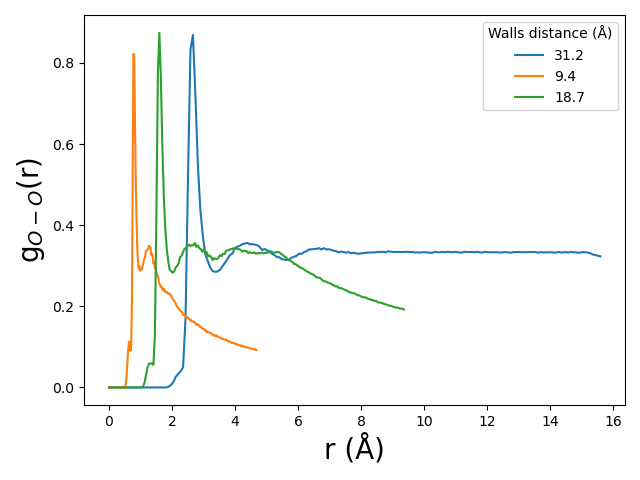
\includegraphics[width=\textwidth]{plotgOO}
	\end{subfigure}
	\begin{subfigure}{0.4\textwidth}
		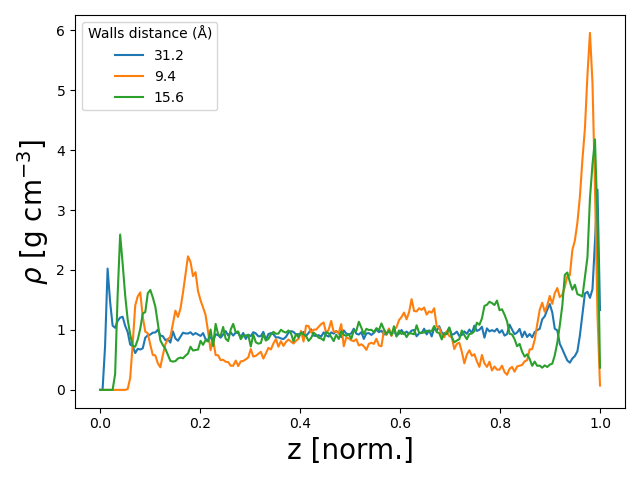
\includegraphics[width=\textwidth]{plot rho}
	\end{subfigure}	
	\caption{(\textit{Left}) Plot of the radial distribution function of the O-O pair and (\textit{Right}) Plot of density profile along \textit{z} for walls sitting at 9.4 \r{A}, 18.7 \r{A} and 31.2 \r{A}.}
	\label{g-rho}
\end{figure}
From g$_{O-O}$ the characteristic wave like structure that is often observed in water is followed by a decay that begins at radii increasing with the distances of the walls.
This last effect is an artifact due to the fact that the spherical crown considered to count the number of oxygen atoms sitting at a particular distance is exceeding the boundaries of the box.
This phenomena becomes visible when not all the sides of the box are equal, which means that when the walls are closer, the effect becomes clearer to see.
\medskip
Considering the behavior of $\rho$, it was chosen to normalize the distance between the walls for each data series in order to allow a clearer vision of the confinement effects on the density profile.
Indeed, when the walls are set to be more than 15 \r{A} from each other, it is possible to identify a stably flat region in the middle where density is roughly 1.
Vice versa, it is observed that when the walls are closing in, the disturbances in density interact.
\medskip
\subsubsection{Self-diffusion}
Self-diffusion properties were assessed along the confined dimension to obtain D$_{z}$(L).
On the left side of Fig. \ref{diffz}, it is possible to appreciate how the mobility of water molecules is reduced when the walls are placed closer to one another.
\begin{figure}[h!]
	\centering
	\begin{subfigure}{0.45\textwidth}
		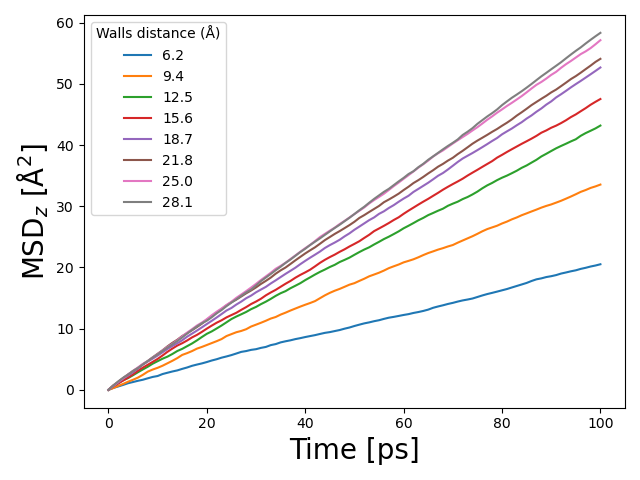
\includegraphics[width=\textwidth]{plot msd}
	\end{subfigure}
	\begin{subfigure}{0.45\textwidth}
		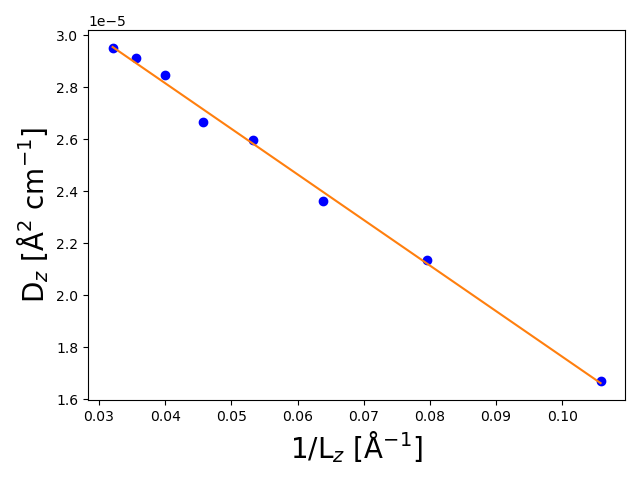
\includegraphics[width=\textwidth]{plot diffz}
	\end{subfigure}	
	\caption{(\textit{Left}) Plot of MSD along \textit{z} over time and (\textit{Right}) Plot of diffusion coefficient against the reciprocal of the distance of the walls.}
	\label{diffz}
\end{figure}
The slope of the Mean Square Displacement (MSD) along \textit{z} is used to calculate the relative diffusion coefficient for each box size.
$D_{z}$ correlates with the reciprocal of the length of the confined dimension, as demonstrated by \citet{yeh_system-size_2004}.
In this case $d = 1$ since the motion on the $x,y$ plane is neglected.
However, in this case the bulk diffusion coefficient estimated is  $D_{0,z} = (3.46 \pm 0.03)\, 10^{-5} \, cm^{2} s^{-1}$ which is an overestimation of the experimental $D_{0} = 2.23 \, 10^{-5}\, cm^{2} s^{-1}$\cite{mills_self-diffusion_1973} by $55\%$.
This could be due to the anisotropy introduced by the presence of the walls.
Since the only components of the displacement that has been considered so far is along $z$, the study has been repeated on the overall MSD, including the brownian motion along the axis $x$ and $y$, to study the anisotropy in diffusion coefficient.
The new diffusion-size correlation was established considering always the $z$ side as the confining one and the plot is depicted in Fig. \ref{diff}.
\begin{figure}
	\centering
	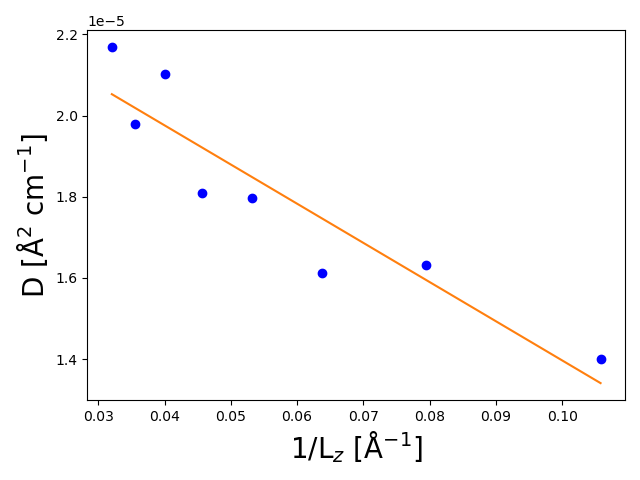
\includegraphics[width=0.6\textwidth]{plot diff}
	\caption{Plot and linear regression of the overall diffusion coefficient of water between two walls placed at different distances.}
	\label{diff}
\end{figure}
In this case, the estimated bulk diffusion coefficient is $D_{0} = (2.36 \pm 0.10)\, 10^{-5} \, cm^{2} s^{-1}$, which is compatible with the experimental value.
This, however must be reconsidered once the diffusion coefficient is split into its components.
Since the only anisotropy is introduced in the system by a Lennard-Jones potential, the diffusion coefficient tensor will be assumed as diagonal, with the terms $D_{xx} = D_{yy} \neq D_{zz}$.
This approach aims at determining the diffusion coefficient on the directions lying on the plane not confined, which will be nominated $D_{x,y} = D_{xx} = D_{yy}$ and can be found by the equation:
\begin{equation}
	D_{x,y} = \frac{3}{2}D - \frac{1}{2}D_{z}
\end{equation}
This calculation leads to $D_{x,y} = (1.81 \pm 0.09)\, 10^{-5} \, cm^{2} s^{-1}$, which is fairly lower than the expected value for an isotropic behavior.
Therefore, it has been proven that the presence of interacting walls doesn't affect the overall diffusivity of the enclosed water, but introduces an anisotropic behavior that privileges the diffusion across the section of the system.
%----------------------------------------------------------------------------------------
\section*{Conclusion}
MD simulations were run on a number of configurations differing solely on the distance between two walls enclosing the water molecules.
The trajectories were validated to satisfy the thermodynamic requirements for a meaningful evaluation of dynamic properties, such as temperature and potential energy.
Furthermore, the effect of walls interaction on water structure was discussed by highlighting the differences of RDF and density profile based on the degree of confinement in which the fluid was constrained.
Ultimately, anisotropy in diffusion coefficient is quantified and imputed to the presence of walls and their interaction with the water molecules is found to promote diffusion along the $z$ axis. 
%----------------------------------------------------------------------------------------

\bibliography{references}
\end{document}
